This section looks at previous work in similar fields. It starts with presenting the paper that offer the idea that this thesis further explores, and then looks at past research on using Twitter and critical infrastructure data for similar tasks. TODO: oppdater denne når kap2 er mer ferdig-ish.

\section{Spatiotemporal information from urban systems}
In the novel study of "Detecting flu outbreaks based on spatiotemporal information from an urban system", which is the base idea for this thesis, Grottenberg et al. \cite{spatiotemp_urban_sys} outlines a design for a system for surveillance of flu outbreaks. Emphasis on the belief that real-time data flows could prove useful in both understanding social functions during disasters and crisis as well as give " ... actionable intelligence for use in influenza management efforts.". The goal would be to extend the already implemented infrastructure with an approach to monitor human behaviour in trends throughout the influenza activity in hope for discrepancies detected through spatial analysis on important measurements. The borrowed figure \ref{fig:grottenberg} from his article sums up what this thesis hopes to accomplish, namely to find a correlation between different datasets and the datasets from the Norwegian public health institution (NIPH), this interference of public behaviour would become visible in essential criterion.
This short read \cite{spatiotemp_urban_sys} is recommended as it gives a more in-depth understanding of the incentive for this thesis.

\begin{figure}[h]
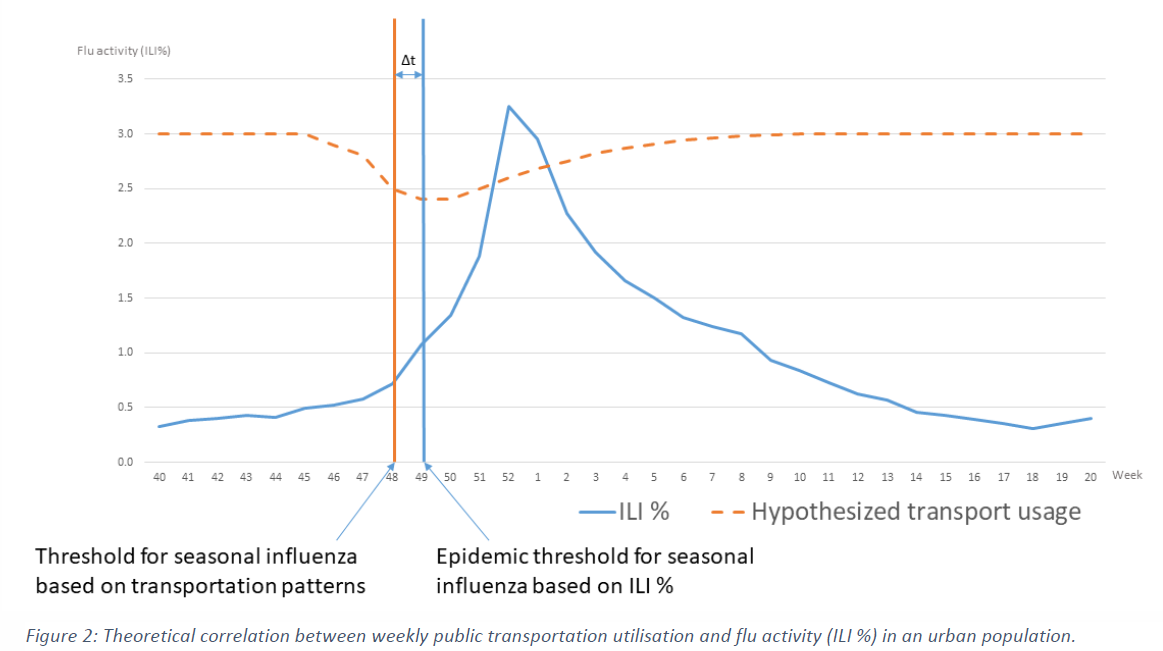
\includegraphics[width=16cm]{grottenberg}
\centering
\caption{Figure from Grottenberg et al. \cite{spatiotemp_urban_sys}}
\label{fig:grottenberg}
\end{figure}

\section{The Ebola epidemic}
The west African Ebola viral haemorrhagic fever (VHF) epidemic lasted from 2013 to 2016 and spread to a wide part of the globe. Ebola causes fever, sore throat, muscular pain, headaches and lastly internal haemorrhage (internal bleeding), the death rate is about 25\% to 95\% with an average of 50\%\cite{who_ebola}. \\Tom Koch\cite{koch2016ebola} with his international journal of epidemiology "Ebola in West Africa: lessons we may have learned" hopes that "... future disease outbreaks in rural areas with minimal resources can be better and more rapidly assessed.". Koch highlights the importance of ecological mapping to spatially identify environmental status that actively encourages disease opulence and expansion. Mapping the terrain and human assets with a geographical positioning system (GPS) provides practical means of ameliorating recurring pandemics. \\An early response to emergency incidents is necessary for efficient containment, and mapping disease contributes to that objective. Koch further describes mapping as an important surveillance spatial tool to identify and contain outbreaks in his commentary "Mapping medical Disasters: Ebola Makes Old Lessons, New"\cite{koch2015mapping}. Knowledge about the location of disease and extent of official health resources provides more time to asses the situation and respond. The 2014 Ebola epidemic failed to survey the seriousness of the outbreak and dreadful events followed. Among the lessons learned from this happening is that the need for detailed medical mapping as soon as possible is paramount for a potential contagion. These technologies matter and are important to implement when resources are met and laid out for, collecting data to serve the public health as a warning system is something to be strived for.\\ During the Ebola disaster in 2014-2015 Médecins Sans Frontières\cite{gis_support} situated devoted Geographic Information Systems (GIS) officers to aid epidemiologists in the creation of topical maps to further support the operation. GIS was greatly beneficial to logistics, epidemiologists, and health promotion by providing knowledge about current disease hotspot flares and acting as a warning system for surrounding districts. Volunteered Geographic Information (VGI) was also used\cite{moeller2015mapping} in mapathons (map creating 'marathons') on the initiative of the American Red Cross in cooperation with the Humanitarian OpenStreetMap Team.\\ With sufficient technological spatial data infrastructure, this process could be automated, and an even more effective emergency management system could be devised. The Ebola outbreak of 2013-2016 goes to show the severity of pandemics, and systems can be developed to effectively combat infectious outbreaks. Even though Ebola is a more serious illness than influenza it goes to show that emergency management systems is sorely needed and have a multitude of applications. Research, development and implementation in many situations overall betters quality and realisation, and the Ebola incident gives insights into managing influenza outbreaks by such systems even in Norway.




\section{Seasonal influenza}
Seasonal influenza, like Ebola, is a recurring disease and has the potential to spread worldwide and thus becoming a pandemic affliction. New undertakes to influenza prevention and treatment management both seasonal and pandemics are beneficial. In their article Catharine Paules and Kanta Subbarao\cite{article_Paules} describes the "... clinical presentation, transmission, diagnosis, management, and prevention of seasonal influenza infection.", and outlines that there are two forms of influenza outbreaks that occur globally: seasonal epidemics caused by type A and type B virus, and sporadic pandemics only caused by type A viruses. Every year the virus undergoes new mutations and "if the novel influenza virus spreads efficiently and sustainable from person to person, it can cause a global pandemic.", making influenza virus a continuous threat to best be dealt with.

In the last hundred years of human history there have been three pandemic influenza outbreaks (in 1918, 1957 and 1968) provoking remarkable mortality. Guan et al.\cite{guan2010emergence} recaps the historical evolutionary pathways of influenza viruses that cause pandemics and suggestions to early detection and control. Perhaps the most known outbreak is the Spanish flu of 1918, only a hundred years ago, which claimed the lives of about 20 million to 50 million human lives worldwide, this virus's origin is considered avian and created the precedence for future pandemics to come. Guan et al. highlights the importance of creating a "... systematic surveillance of influenza in pigs that will provide early evidence for mixing of new genetic elements and the emergence of viruses with pandemic potential in humans.". World Health Organization (WHO) pronounce in their "Pandemic H1N1 2009"\cite{world2009pandemic} report that the H1N1 virus (the Spanish flu) "... emerged almost simultaneously from birds into humans and swine.". They also describe how pandemics function in waves, being more mild in the beginning and increasing in gravity into the second wave.

There are numerous studies that examines the individual behaviour and their effect on spreading influenza. Karimi et al.\cite{karimi2015effect} creates an agent based model to simulate controlling spread of infectious diseases by surveying behaviour and importance of vaccination and social distancing. They claim that other studies fail to take into account ... "self-initiated protective behaviors that individuals develop in the face of an infectious disease.". Their paper demonstrates how agent based simulation may be employed "... to study influenza outbreak and assess various prevention strategies.". Kerckhove et al.\cite{van2013impact} also describes how influenza-like illnesses influences individual social mixing patterns, and they express that people when showing symptoms of influenza have fewer social encounters. 
They conclude that "... identifying, treating, and isolating symptomatic individuals should be the focus of public health efforts in order to prevent transmission to others in the community.".

Surveillance of influenza can be done on an individual level as well as societal. Xu et al.\cite{xu2014surveillance} describes this on a personal level and concludes with the value of continuously monitoring high risk behaviours, chronic conditions, and generally adopting and promoting a "healthy lifestyle", particularly in individuals with elevated risk of being infected with influenza. Dikic et al.\cite{dukic2012tracking} describes how to track influenza epidemics with Google's flu trends\cite{google_flu_trends} data and a state-space SEIR model. Public health officials rely on surveillance data to track, estimate and finally ameliorate the effects, improving their information flow is highly favourable. Search engine activity has dramatically increased over the last decades and Google employ advanced algorithms to predict the trajectory of influenza-like illness (ILI) trends by users searching for ILI keywords. Dikic et al. concludes with the potential "... for developing real-time surveillance mechanisms." with the ever growing computer programs and insight to clever algorithms to better serve such a system.

Developing an analytic disease management system based on societal data seems to be a new emerging technological possibility that can have considerable positive effects for the well being of all of humanity's prosperity and global development.






\section{Data management and critical infrastructure}
This thesis touches upon data management and development of crisis response systems. The proposed system would act as a tool in a larger system in the development of support decision making in the event of an epidemic influenza preparedness and outbreak. 

Responding to extensive crisis or disasters requires coordination between a multitude of relief agencies, and this demands the right information at the right time. A system that can detect an emergence of a possible influenza outbreak would be an aiding factor to this. Gonzales et al. \cite{gonzalez2009framework} goes into general details of how the quality of information during a crisis response is important and how to better coordinate relief agencies with the right information at the right time. Their report includes a case study where simulation of interagency crisis response by the port of Rotterdam in the Netherlands, in particular this case study emphasise the qualitative trial and strategy throughout interagency crisis management. Extensive emergencies requires involvement of a multitude of relief and other regional service assets to cooperate and share relevant and timely information. The specifics of the case study simulates the collision of a containership with a passenger ship where the containership explodes and leaks hazardous chemicals. Responding to such a catastrophic tense event requires cooperation of multiple authorities from professional representatives guided by regional and port experts. Gonzales et al. concludes that designing a computer based system for management and automation services of a work flow information conductor would better the over all quality of response and guidance. The system proposed by this thesis could be a module of such a system. 

Machine-learning algorithms may also be of use in spatiotemporal analysis of social media data for disasters and damage assessment. Resch et al \cite{resch2018combining} explains how the current management of disasters have several shortcomings that can be solved by machine-learning topic models and spatiotemporal analysis. Temporal lags and limited resolution of information prevents successful and accurate resource deployment, advantages of new approaches with real-time collecting of data, like social media and other crowdsourcing networks "can significantly improve disaster management". Resch et al proposes a new approach to analyse social media with the combination of semantic machine-learning algorithms with spatio and temporal analysis. The challenge is detecting data flow continuously without prior analysis and knowledge about the event in question. Their results show remarkable improvement to accurate event tracking and other hotspots, disaster management and valuable insight to affected regions and assets.

Simulation modules could also be added to this system. This thesis is not a simulation tool but it is worth mentioning that there are several such proposed models of influenza and other disease simulation implementations. Shao et al. \cite{shao2016forecasting} ask the question of whether it is possible by monitoring public urban data by designing a social network sensor for epidemics to predict the coming outline of an overall epidemic, and simulates this. Developing sufficient heuristics in order to adpot social sensors to forecast influenza outbreaks when probabilistic views of structure of simulated influenza propagations interests public health dignitaries and govermental stratagem designers. There are many more simulation tools, another is proposed by Stein et al. \cite{stein2012development} which models an influenza outbreak in two provinces of Lao. Stein et al's framework proposes that planning for influenza outbreaks is an exigent engagement that requires predictive models to better evaluate responsive strategies. Stein et al freely offers their simulation too called AsianFluCap on their website and describes it as ".. a user-friendly, comprehensive and flexible simulation tool which can be used by decision makers involved in pandemic preparedness to estimate and compare the impact on health care resource capacity during different pandemic scenarios.". Simulations are a way of preparing and training in order to reveal flaws and evaluation of response plans and deployment of limited health care resources, and raise awareness of surges in sudden resource demands during pandemics, especially so where such resources are scarce and efficient delegation is important.


\section{Open source and Collection Intelligence}
In this section description of volunteered or otherwise open source publication, datasets and investigation of influenza and other infectious diseases are described.

\subsection{Spatiotemporal information from VGI}
Volunteered Geographic Information (VGI) is peer-produced crowd spatial data for use in crisis responses. Mobilizing digital volunteers to help with disastrous events alleviates the data needed by relief agents, VGI is peer-produced spatial data that is highly up-to-date. In 2010 the Haiti Earthquake levelled many official government buildings and with them access to official mapping resources\cite{palen2015success}. In just a few days volunteers contributed to OpenStreetMap\cite{OpenStreetMap} (OSM) and created an even better map of Haiti using satellite images by individually identifying map resources. A similar approach was initiated during the 2015 Nepal earthquake\cite{hu2016task}. Anderson et al\cite{anderson2018crowd} describes methods for evaluating the quality of VGI and to the development of "... rapid metrics of quality for digital data generated under socially distributed conditions ...". They reason that peer production platforms will be a more integrated part of disaster management and that when the risk of lives and infrastructure is present a solid basis for quality control of VGI information should be established whenever VGI is used.





\subsection{Google flu trends}
Google Flu Trends (GFT) exploit aggregated search data to approximate influenza-like illnesses (ILI) in real-time. People search for health related information online, and Google is a search engine used for this motivation, and there are more flu related searches when people become infected with influenza during the flu seasons. Certain search terms are better correlated with ILI, and Google with the help from the USA Centers for Disease Control and Prevention\cite{CDC} uses analytical algorithms and CDC's ILI data to match the best corresponding search queries/terms. The information derived becomes real-time as data is firstly presented to Google via users search queries before CDC acquires that same data though their means. GFT also works in the same manner in other countries, except they are labeled experimental because they cannot be compared with ILI data as such information is often inaccessible to Google. Google aslo filter out terms that are made popular by media thus creating a surge for those queries/terms. GFT was created in 2008 and was only operational until 2014, it was discontinued because of failed predictions and lack of coupling with scientific research, it is was however a promising and interesting use of big data analysis.


  

\subsection{Strava}
Strava\cite{strava_main} is a website and a mobile application that is used by athletes or other persons that enjoy outdoor cardiovascular exercises. It track users by a global positioning system (GPS) and users can then upload this data to their profiles\cite{strata_wiki}. Datasets gathered by Strava are available to other services, and aggregated logs may be used to derive different information. In the instance of tracking influenza, results about when the population's interest for such activity declines could be an indicator of ILI. 





\subsection{Twitter}
"Twitter is an online news and social networking service on which users post and interact with messages known as "tweets"."\cite{twitter_twitter}. A number of studies have been performed on the information that the users of Twitter generate. These studies analyse millions of tweets to extract aggregate information. Researchers have studied tweets to reveal political opinions\cite{twitter_politic}, measure public health\cite{twitter_flu_trends}, linguistic sentiments\cite{twitter_linguistics} and even environmental phenomena such as earthquakes\cite{twitter_earthQuake}. Achrekar et al.\cite{twitter_flu_trends} examines tweet flu trends and compares them with actual influenza data. The results show a high correlation between self-reported instances of flu-like illnesses (ILI) and reported ILI by public health providers. Achrekar references claims that early prevention limits the spread of infectious diseases and that twitter data is an 'untapped data source' that actually is quite reliable. Another report by Byrd et al.\cite{byrd2016mining} also evidence how Twitter surveillance and classifying tweets by sentiment characterstics exactly identify users with ILI symptoms in selected cities in real-time, and also speculates usage of this technology in application of other disease protection systems. This demonstrates how social media can be  used to predict real-world consequences, and gives credibility to usage in this thesis. \\Michal J. Paul and Mark Dredze \cite{twitter_what_you_tweet} also conducted research on the usage of twitter data to measure population characteristics. In their conclusion twitter data from many users divulges reliable information about a certain topic of interest and in particular public health. They further discuss the pros and cons namely that self-reported is low cost and rapid transmission, whereas on the other side this is a 'blind authorship, lack of source citation and presentation of opinion as fact'. Certainly twitter messages may be false on an individual level, but however when taking into account thousands or even millions of messages this seems not plausible on a bigger scale. Albuquerque et al. \cite{de2015geographic} describes how they were able to extract useful information via twitter to better acquire information about a flood phenomena in German rivers, and combining this with authoritative data for disaster management. They write that social media messages gives a valuable and useful information to further aid and manage disasters as an addition to other sources , in a way this is practically the same as asking volunteers for help. For these reasons twitter data is used in this thesis as it proves an interesting and unique source of relevant information.





